% !TEX encoding = UTF-8 Unicode
%% 
%%  This file is asmejour-template.tex, a template to format papers in the style of ASME journal papers 
%%  as they are being published in 2020.
%%
%%  This file is version 1.12 dated 2020/04/12
%%
%%  Author: John H. Lienhard V
%%          Department of Mechanical Engineering
%%          Massachusetts Institute of Technology
%%          Cambridge, MA 02139-4307 USA
%%
%%  Class options are set up in the asmejour.cls file. These include:
%%
%%          * Option to color the vertical bar in the title block [barcolor = colorname] 
%%          *    where colorname is any name def'd by xcolor package; omit barcolor option to get black
%%
%%          * Option to omit the list of figures and list of tables [nolists]
%%
%%          * Math options from M. Sharpe's newtxmath package: upright integrals [upint]; and
%%          *    varvw for a v and w that are better distinguished from greek nu; and also 
%%          *    smallerops, varg, slantedGreek, frenchmath, varbb, cmbraces. Version 1.5 or higher
%%          *    is recommended.
%%
%%          * Option to include line numbers [lineno]. The lineno package does not number tables, 
%%          *    footnotes, captions, etc. You must run *twice* for proper placement of the numbers. 
%%          *    This option will disable balancing of the column heights on final page.
%%
%%			* Option to balance column heights on final page [balance]. This option sometimes
%%			*    misbehaves, so use it with an awareness that it can create unexpected problems.
%%			*	 This option is not compatible with line numbering.
%%
%%          * Many options for calligraphic, script, and fraktur fonts from the mathalfa package; the
%%          *    example value used is: mathalfa=cal=euler (use Euler font for \mathcal)
%%          *    some other options for cal are: dutchcal, zapfc, cm (default), boondox,...
%%          *    frak (fraktur), bb (blackboard bold), scr (script) may also be controlled.
%%
%%          * An option to omit all the ASME text fields from the footer [nofoot].
%%
%%          * An option to omit only the ASME copyright field from the footer [nocopyright].
%%
%%          * An option to use newtxtext's superiors font for footnotes [nodefaultsups] and an option
%%          *    for slightly larger small capitals, largesc
%%
%%          * Options to set (for the babel package) a primary language [lang= ], and secondary or tertiary
%%          *    languages, [lang-second] and [lang-third].  If no option is given, english is the main language.
%%			*	 If a secondary or tertiary language is selected, a primary language must also be specified.
%%
%%          * Option to allow hyphenation of the typewriter font [hyphenate]
%%          *    Hyphenation is normally suppressed for typewriter mode because it is often used for code.
%%
%%  For details of newtxmath and mathalfa, refer to their documentation (available on CTAN: http://ctan.org).
%%
%%  The use of commands defined or modified by the asmejour class is illustrated below. In particular, 
%%  some care is needed when using complicated math and macros in section headings, 
%%  to avoid problems with pdf bookmarks, which is facilitated by the optional argument of \section, 
%%  as also illustrated below.
%%
 %=========================================================
%% 
%% LICENSE:
%%
%% Copyright (c) 2020 John Lienhard
%%
%% Permission is hereby granted, free of charge, to any person obtaining a copy of this software and 
%% associated documentation files (the "Software"), to deal in the Software without restriction, 
%% including without limitation the rights to use, copy, modify, merge, publish, distribute, sublicense, 
%% and/or sell copies of the Software, and to permit persons to whom the Software is furnished to do so, 
%% subject to the following conditions:
%%
%% The above copyright notice and this permission notice shall be included in all copies or 
%% substantial portions of the Software.
%%
%% The software is provided "as is", without warranty of any kind, express or implied, including but 
%% not limited to the warranties of merchantability, fitness for a particular purpose and noninfringement. 
%% In no event shall the authors or copyright holders be liable for any claim, damages or other liability, 
%% whether in an action of contract, tort or otherwise, arising from, out of or in connection with the 
%% software or the use or other dealings in the software.
%%
%%%%%%%%%%%%%%%%%%%%%%%%%%%%%%%%%%%%%%%%%%%%%%%%%%%%%%%%%%%%%%%%%%%%%%%%%%%%%%%%%%%%%%%%%%%%%%%%%%%%%%%


%% Class options are described above.
\documentclass[largesc,upint,varvw,barcolor=Red4,nocopyright,hyphenate,balance,lang-second=french,lang=english]{asmejour}

%%%%%  FIELDS TO BE COMPLETED FOLLOW  %%%%%%%%%%%%%%%%%%%%%%%%%%%%%%%%%%%

%%%%%  pdf metadata, the user should edit %%%%%%%%%%%%%%%%%%
\hypersetup{%
	pdftitle={ASME Journal Paper Template},                % <=== change to YOUR pdf file title
	pdfkeywords={ASME, Paper, Template, LaTeX, BibTeX, asmejour class},    % <=== change to YOUR pdf keywords
	pdfauthor={John H. Lienhard},                          % <=== change to YOUR name[s]!!!
}

%%%% Journal name and optional copyright year %%%%%%%%%%%%%%

%% Omit "Journal of"
%% If Journal Name is quite long, use \\ to insert a line break
\JourName{Heat Transfer} %<=== change to name of your journal

\PaperYear % defaults to current year if no argument given or if command is omitted; 
           % \PaperYear{} omits year; \PaperYear{2018} sets 2018.
                   
%%%%%%%%%  End of Preamble  %%%%%%%%%%%%%%%%%%%%%%%%%%%%%%%%%

\begin{document}

% Change to your author name[s] and addresses, in the desired order of authors.
% First name, middle initial, last name
% Use title case (upper and lower case letters)
% Note usage below for corresponding author.

\SetAuthorBlock{Author Name[s]}{Department of Mechanical Engineering,\\
   Institution or Company Name,\\
   Street address,\\
   City, State, Country \\
   email: xxx@yyy.zzz} 

% To label one or more corresponding authors put "Name\CorrespondingAuthor". No space after "Name".
% An optional argument can be added if email is not in address block as
%      "Name\CorrespondingAuthor{write@to.me}"
% Can also include multiple emails and use the command more than once for multiple corresponding authors,
%      "Name\CorrespondingAuthor{write@to.him, write@to.her}"

\SetAuthorBlock{John H.\ Lienhard V\CorrespondingAuthor}{%
Rohsenow Kendall Heat Transfer Laboratory, \\
Department of Mechanical Engineering,\\
Massachusetts Institute of Technology, \\
Cambridge, MA 02139 USA \\
email: lienhard@mit.edu
}

%%% Change to your paper title. Can insert line breaks if you wish (otherwise breaks are selected automatically).
\title{Preprint Template for ASME\\ Journal Papers:  asmejour.cls}


%%% Change these to your keywords.  Keywords are automatically printed at the end of the abstract.
%%% This command must come BEFORE the end of the abstract.
%%% If you don't want keywords, delete the command.
\keywords{ASME, Paper, Template, {\upshape\LaTeX}, {\upshape\hologo{BibTeX}}}
 
   
%% Abstract should be no more than 250 words
\begin{abstract}
This paper is an example and template for the {\upshape\texttt{asmejour}} class. Papers typeset in this class will follow ASME journal style for margins, fonts, headings, captions, and reference formats. Standard {\upshape\LaTeX} commands are used. The class will lay out the author, title, and abstract in ASME style. The class will produce a pdf file that that includes hyperlinks, bookmarks, and pdf metadata. The class is intended to be used with the {\upshape\texttt{asmejour.bst} \hologo{BibTeX}} style for typesetting references, which is part of this distribution.  This style supports hyperlinks and modern reference formats, following current ASME practice. The class may be invoked with several options, most of which address math fonts. The class calls a number of packages, all of which are in {\upshape\TeX~Live} and in CTAN (\href{http://ctan.org}{ctan.org}). The class is compatible with {\upshape\hologo{pdfLaTeX}} or {\upshape\hologo{LuaLaTeX}}.
\end{abstract}


\date{Version \versionno, \today} %% can modify this information as desired. 
							%% Putting \date{} will suppress any date.  
							%% If this command is omitted, date defaults to \today
							%% This command must come somewhere before \maketitle

\maketitle %% This command creates the author/title/abstract block. Essential!

%%%%%%%%%%%%%%%%%%%%%%%%%%%%%%%%%%%%%%%%%%%%%%%%%%%%%%%%%%%%%%%%%%%%%%%%%%%%%%%%%%%%%%%%%%%%%%%%%%%%%%%
%%%%%%%%%%%%%%%%%%%%%  End of fields to be completed. Now write! %%%%%%%%%%%%%%%%%%%%%%%%%%%%%%%%%%%%%%


\section{Introduction}

The \texttt{asmejour} class file will typeset papers with margins, fonts, headings, captions, and reference formats that follow those used in journals published by the American Society of Mechanical Engineers (ASME). Internal and external hyperlinks will be set automatically, and the pdf file will contain bookmarks and metadata.

This class is not a publication of ASME. The intended use of this package is to allow authors to format their papers in ASME style prior to submission to an ASME journal for peer review.

The \texttt{.tex} file may be written using standard \LaTeX\ commands, although some specific initial commands are needed to format the block containing the author[s], title, and abstract.

\subsection{Essential Initial Commands}
To begin, fill in the fields to be completed at top of the \texttt{asmejour-template.tex} file. The pdf metadata will be placed into the pdf file itself. 

For each author, put author names and affiliation (with line breaks) into a separate \verb|\SetAuthorBlock{name}{affiliation}| command; follow the syntax illustrated \texttt{asmejour-template.tex} file.  One author (or more) may be designated as the corresponding author  by placing the command \verb|\CorrespondingAuthor| at the end of that name.  

The title should be placed into \verb|\title{..}|, and line breaks may be specified if desired. Keywords may optionally be including using the \verb|\keywords{..}| command; this command \textit{must} be issued before the abstract. The abstract text must be placed into \verb|\begin{abstract}|\ldots\verb|\end{abstract}|. The abstract will automatically be italicized. 

The date is given as an unnumbered footnote, which deafults to \verb|\today|. Other text for \verb|\date{..}| may be specified. Putting \verb|\date{}| will suppress the footnote.

After setting up the authors, title, and abstract, issue the \verb|\maketitle| command. 

\subsection{Optional to the Color Title Bar}
The vertical bar in the title block is black in all ASME journals. Since the \texttt{asmejour} class is only for preprints, we include the [fun] option to have the bar in color. Any color \texttt{name} recognized by the \texttt{xcolor} package may be invoked by including the option \texttt{barcolor=name} in the \verb|\documentclass[..]{asmejour}| command. The color name is \texttt{Red4} by default. (To have a black bar, either omit the option entirely or use the name \texttt{black}.)


%%%%%%%%%%%%%%%%%%%%%%%%%%%%%%%%%%%%%%%%%%%%%%%%%%%%%%%%%%%%%%%%%%%%%%
\section{References to Figures, Equations, and Citations}

For ASME papers, the labels Figure and Equation should be abbreviated when they do not start a sentence, as in Fig.~\ref{fig:1} and Eq.~\eqref{eqn:1}. Figure~\ref{fig:1} is spelled out when it starts a sentence. Equation~\eqref{eqn:1} is spelled out when it starts a sentence. 

Citations will be numbered automatically \cite{DKE1969}. They should be inserted at the appropriate point using a \verb|\cite{ref}| command~\cite{toohey2007,gibson2008}. The citations will be automatically sorted and compressed, as well, if they are given in a set \cite{stevens1999, DKE1969, wions2006, oligaria2011, mollen2014, smith2014, apple2019}. If naming a reference explicitly, use an abbreviation in front of the number, as in Ref.~\cite{smith2014}. Reference~\cite{smith2014} is appropriate at the beginning of a sentence.
See the \texttt{asmeconf-sample.bib} file for examples of how to enter your references.

Equations are typeset in the usual way.  The class file loads the \texttt{amsmath} and \texttt{mathtools} packages. Further, the \texttt{newtxmath} package used for the math fonts includes many additional features.
\begin{equation}\label{eqn:1}
\mathbf{q} = -k\nabla T
\end{equation}


%%%%%%%%%%%%%%%%%%%%%%%%%%%%%%%%%%%%%%%%%%
\section{Section Headings and Captions}

ASME requires that section headings and captions be set in bold face. In addition, the captions must be in sans serif type. The \texttt{asmejour} class will do this automatically.  You can place \verb|\cite{..}|, \verb|\ref{..}|, \verb|\label{..}|, and into headings and captions directly, as you would in the main text.  You can place \verb|\footnote{..}| into headings, but not into captions.\footnote{See \texttt{tex-stackexchange} for various approaches to footnotes in captions, if they seem necessary. For footnotes in tables, use the \texttt{tablefootnote} package.}

Sections may either be numbered or left unnumbered. ASME publishes papers in either style.

Math can be used in either captions or section headings, and an appropriate math font will be automatically selected. For a section heading that includes complicated math (and macros), you may use the optional argument of \verb|\section[..]{..}| to create a pdf bookmark without losing characters or producing warnings or errors. See the \texttt{asmejour-template.tex} source file for examples of this. These bookmarks should usually be text expressions, although some math is supported.  

If you wish to override the default math format in a heading or caption, put \verb|\mathversion{normal}| in the heading or caption. (The \texttt{newtxmath} package \cite{sharpe1} includes a complete set of bold math fonts, however, so the need to override should be rare.)

Single-sentence captions should not end with a period. Multi-sentence captions do include periods.

\subsection{Subsection Headings}
Section, subsection, and subsubsection headings should be in title case (first letter of primary words capitalized). ASME does not use \verb|\paragraph|, so the class file treats this commands like \verb|\subsubsection|. 


%%%%%%%%%%%%% begin figure %%%%%%%%%%%%%%%%%

%% captions go below figures
\begin{figure}
\centering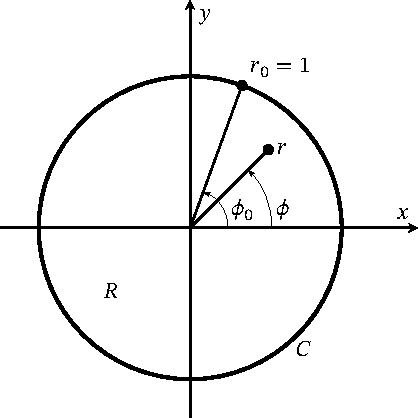
\includegraphics[width=0.7\linewidth]{sample-figure-1.pdf}
\caption{A figure caption with math, Eq.~\eqref{eqn:1}: $z = (r,\phi)$ \cite{Lienhard2019b}\label{fig:1}}
\end{figure}
 
%%%%%%%%%%%%% end figure %%%%%%%%%%%%%%%%%%%


%%%%%%%%%%%%%%%%%%%%%%%%%%%%%%%%%%%%%%%%%%%%%%%%%%%%%%%%%%%%%%%%%%%%%%
\section{More on Math}

To get bold math outside of the captions, you can use the \verb|\bm{..}| macro from the \texttt{bm} package, which is loaded by the class.

\begin{equation}
\bm{ S = k \ln w}
\end{equation}

Math italics are used for roman and lower-case greek letters by default.  If you want an upright letter in math, you can use the relevant math alphabet, e.g., \verb|\mathrm, \mathbf, \mathsf|:
\begin{equation}\label{eqn:newton2}
\vec{F} = m \vec{a} \quad\textrm{or}\quad \vec{\mathrm{F}} = m \vec{\mathrm{a}} \quad\textrm{or}\quad \mathbf{F} = m \mathbf{a} \quad\textrm{or}\quad \vec{\mathsf{F}} = m \vec{\mathsf{a}}
\end{equation}

ASME typesets vectors in upright bold, like the third instance in Eq.\ \eqref{eqn:newton2}, and sets matrices in bold italic. In the next equation $\mathbf{w}$ is a vector and  $\bm{J}_1$ is a matrix:
\begin{equation}\label{eqn:dw}
d\mathbf{w} =
   \begin{pmatrix}
 	du \\ dv
   \end{pmatrix} = 
   \underbrace{\begin{pmatrix}
	 \partial u/\partial x &  \partial u/\partial y \\
	 \partial v/\partial x &  \partial v/\partial y
   \end{pmatrix}}_{=\,\bm{J}_1}  \begin{pmatrix}
 	dx \\ dy
   \end{pmatrix} 
\end{equation}

The \texttt{newtxmath} package includes a large number of options for mathematics, most of which can be called as options to \verb|\documentclass|. For example, the \texttt{upint} option of \texttt{newtxmath} selects upright integral signs (rather than slanted integral signs):
\begin{quote}
\verb|\documentclass[upint]{asmejour}|. 
\end{quote}  
These math options are discussed further in the \texttt{asmejour-template.tex} file. 

In addition, many options for calligraphic, script, and fraktur fonts are available as options to the \texttt{mathalfa} package, which is also loaded. These may be invoked, for example, as 
\begin{quote}
\verb|\documentclass[mathalfa=cal=euler]{asmejour}| 
\end{quote}
which selects the Euler font for \verb|\mathcal| (this is our default). To find all the font options, refer to the \texttt{mathalfa} package documentation \cite{sharpe2}.

The typewriter font loaded is \texttt{inconsolata} (which is sans serif), as suggested by the \texttt{newtx} package documentation. The class is not set up for use with the \texttt{fontspec} or \texttt{unicode-math} packages.


\subsection{Units and Nomenclature} ASME requires SI units. U.S.\ style units may be follow in parentheses. Be sure to put your symbols into the nomenclature list, including the SI units.


%%%%%%%%%%%%%%%%%%%%%%%%%%%%%%%%%%%%%%%%%%%%%%%%%%%%%%%%%%%%%%%%%%%%%%
\section{Tables and Figures}

Table \ref{tab:1} is an example of a simple table. Table captions should be placed above tables.
The class loads the \texttt{array} and \texttt{dcolumn} packages which provide extended capabilities for columns in the \texttt{tabular} environment (used in Tables \ref{tab:2} and \ref{tab:3}). Table~\ref{tab:3} is designed to have exactly the width of a text column. 

The \texttt{booktabs} package \cite{fear} is loaded (and customized) to provide versions of \verb|\toprule|, \verb|\midrule|, and \verb|\bottomrule}| appropriate to ASME-style tables.

Table~\ref{tab:4} shows a table that spans both text columns. Figure~\ref{fig:2} shows a figure spanning both columns. Two column tables and figures will always float to the top of a later page. Subframes in figures, such as  Fig.~\ref{fig:interior-region}, may be referenced individually.

Text in the figures should be checked for legibility at either single-column width (about 83~mm) or full-column width (about 170~mm).  Figure captions should be placed below figures. Images in figures are handled by the standard \texttt{graphicx} package.

Landscape figures and tables may be produced at full-page size by putting \verb|\usepackage[figuresright]{rotating}| in your \texttt{.tex} file's preamble and using the \texttt{sidewaystable*} and \texttt{sidewaysfigure*} environments~\cite{fairbairns}.

%%%%%%%%%%%%%%% begin simple table %%%%%%%%%%%%%%%%%%%%%%%%%% 

%% captions go above tables

\begin{table}[t]
\caption{A simple table\label{tab:1}}
\centering{%
\begin{tabular}{l l r}
\toprule
Experiment & $u$ [m/s] & $T$ [\textdegree C] \\
\midrule
Run 11 & 12.5 & 103.4 \\
Run 12 & 24   & 68.3 \\
\bottomrule
\end{tabular}
}%
\end{table}

%%%%%%%%%%%%%%%% end table  %%%%%%%%%%%%%%%%%%%%%%%%%%%%%%%%%%%% 


%%%%%%%%%%%%%%%%%  begin two column figure  %%%%%%%%%%%%%%%%%%%%%%%%%%%

\begin{figure*}[t]
\begin{subfigure}[t]{0.5\textwidth} % You will get same result using \begin{minipage}[t]{0.5\textwidth}
\vbox{
\vspace*{1.7em}
\centering{
  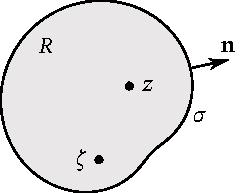
\includegraphics{sample-figure-2a.pdf}
}
\vspace*{1.7em}
}
\subcaption{Interior region\label{fig:interior-region}}
\end{subfigure}%
%%%%%%%% don't leave a break here
\begin{subfigure}[t]{0.5\textwidth} % You will get same result using \begin{minipage}[t]{0.5\textwidth}
\centering{
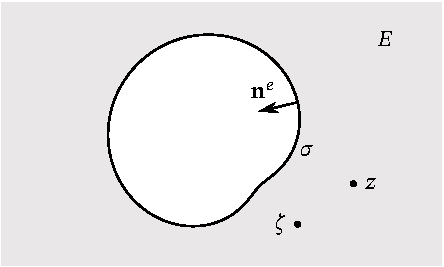
\includegraphics{sample-figure-2b.pdf}
\subcaption{Exterior region\label{fig:exterior-region}}
}\end{subfigure}%
\caption{A figure with two subfigures \cite{Lienhard2019b}\label{fig:2}}
\end{figure*}

%%%%%%%%%%%%%%%%%%%  end two column figure  %%%%%%%%%%%%%%%%%%%%%%%%%%%%%

%%%%%%%%%%%%%%%%%%%%%%%%%%%%%%%%%%%%%%%%%%%%%%%%%%%%%%%%%%%%%%%%%%%%%%
\section{Reference Formatting with \texttt{asmejour.bst}}

The {\upshape\texttt{asmejour.bst}} \hologo{BibTeX} style follows the reference styles observed in ASME journals in early 2020. The vast majority of published references are to journal papers and books. Examples for these and many other entry types are given in the \texttt{asmejour-sample.bib} file, which is part of this distribution. Citations and references are managed by the standard \texttt{natbib} package.
Nevertheless, a few comments are necessary. 

\subsection{Hyperlinked Titles and Numbers} When the entries \verb|@article{..|, \verb|@book{..|, \verb|@inbook{..|, \verb|@incollection{..|, \verb|@proceedings{..|, or \verb|@techreport{..| include \verb|doi={..}|, the document title, paper number, or report number will be hyperlinked to that doi number, and the doi number will not be printed. If no doi is included, but a url or eprint is included, then the title will be hyperlinked to that url or eprint. To display the doi (or the url or eprint when no doi is given), put it into the \verb|note={..}| field (using \verb|\doi{..| or \verb|\url{..| ):
\begin{quote}
\verb|note = {\doi{10.1115/1.4042912}}|
\end{quote}
Include doi numbers in references whenever possible.

\subsection{eprint Support} Elementary support for \texttt{eprint} numbers is included, either hyperlinking or generating a url at the end of the citation. The \texttt{archive} type may be specified using the macros \texttt{arxiv, googlebooks, hndl, jstore, oclc}, or \texttt{pubmed} (e.g., \texttt{archive=hndl},  \textit{without} braces). Both \texttt{eprint} and \texttt{archive} fields \textit{must} be given. Other root urls may be invoked using \verb|archive = {http://another.url.org/}|.

\subsection{Online Sources} A bibliography field \verb|@online{..| is included for citation of online sources, such as web pages. A \texttt{url}, \texttt{doi}, or \texttt{eprint} with \texttt{archive} should be included. See the examples of use in the \texttt{asmejour-sample.bib} file. 

\subsection{Date Accessed} The \verb|urldate={..}| field may be used to provide the date on which a given url was accessed. By default, the text printed will be \texttt{accessed `date',}. The word ``accessed'' may be changed using the \verb|urltype={..}| field.

\subsection{Conference Location and Date} For the entry types \verb|@inproceeedings{..| and \verb|@proceeedings{..|, you may include \verb|venue={..}| and \verb|eventdate={..}| to specify the city and the date of a conference. Omit \verb|address={..}| if \verb|venue={..}| is used.

\subsection{Version Number\protect\footnote{Footnotes can appear in \texttt{\string\section} commands. However, when the \texttt{[lineno]} option is used either: i) write \texttt{\string\protect\string\footnote\{..\}}; or ii) include the optional argument, as in \texttt{\string\section[Foo]\{Foo\string\footnote\{..\}\}}.\label{ftnt:3}}} 
The \verb|version={..}| field may be used with \verb|@book|, \verb|@online|, and \verb|@manual|. By default, the text will read \texttt{Version `number'} as in Refs.~\cite{sharpe1,sharpe2},  but different wording may be selected using the \verb|versiontype={..}| field, to have ``Revision''  or something similar, as in Ref.~\cite{GSL}. ASME often puts the version in the title, as in Refs.~\cite{dlmf, texshop}, so I've left the final decision for discussion between the authors and the copy editor.

\subsection{Capitalization of Titles} ASME's bibliography style requires that titles be in title case. The first letters of principal words are capitalized. This must be done when writing the \texttt{.bib} file.
%(ASME capitalizes ``With'', but not other prepositions).

\subsection{Articles in Collections} In addition to the standard entry, \verb|@incollection{..|, an entry  \verb|@inserialcollection{..| is defined for serials in which each volume has a different title. See the \texttt{asmejour-sample.bib} file for discussion and compare Ref.~\cite{clauser56} to Ref.~\cite{DKE70}.


%%%%%%%%%%%%%%% begin more complicated table %%%%%%%%%%%%%%%%%%%%%%%%%%%%%%%%%%%%

\begin{table}[t]
\caption{Table with more complicated columns}\label{tab:2}%
\centering{%
\begin{tabular}{!{\hspace*{0.5cm}} >{\raggedright\hangindent=1em} p{3cm} d{3} @{\hspace*{1cm}} d{3} !{\hspace*{0.5cm}}}
\toprule
Experiment & \multicolumn{1}{c@{\hspace*{1cm}}}{$u$ [m/s]} & \multicolumn{1}{c!{\hspace*{0.5cm}}}{$T$ [\textdegree C]} \\
\midrule
The first experiment we ran this morning   & 124.3     &   68.3  \\
The second experiment we ran this morning  &  82.50    &  103.46 \\
Our competitor's data                      &  72.321   &  141.384\\
\bottomrule
\end{tabular}
}%
\end{table}

%%%%%%%%%%%%%%%% end table  %%%%%%%%%%%%%%%%%%%%%%%%%%%%%%%%%%%% 


%%%%%%%%%%%%%%%%%%%%%%%%%%%%%%%%%%%%%%%%%%%%%%%%%%%%%%%%%%%%%%%%
\section{Additional Options for \texttt{asmejour.cls}}
The class accepts a number of options in addition to those already described.

\subsection{Lists of Figures and Tables} A list of figures and a list of tables are generated automatically as the last page.  To omit these lists, use the option \texttt{[nolists]}.

\subsection{Final Column Balancing} The option \texttt{[balance]} invokes the the \texttt{flushend} package~\cite{tolusis}.
This package will attempt to give equal height to the two columns on the last page. The performance of this package is sometimes inconsistent (with odd page layout or, very rarely, errors), so use this option with caution.

\subsection{Line Numbers} The option \texttt{[lineno]} invokes the the \texttt{lineno} package~\cite{bottcher}.  This will produce line numbers in the margins. You must run \LaTeX\ twice for proper placement of the numbers. The \texttt{lineno} package is not compatible with the \texttt{flushend} package that makes final short columns the same height. Balancing is disabled when this option is called. See the documentation of the \texttt{lineno} package for further commands to control line numbering. See footnote~\ref{ftnt:3} with regard to footnotes in section headings while this option is in~effect. The abstract, tables, captions, and footnotes will not be numbered.

\subsection{Changing the Footer Text}\label{sec:footer} The option \texttt{[nofoot]} will omit everything other than a page number from the page footer.  The option \texttt{nocopyright} will omit the ASME copyright from the first page footer. The command \verb|\PreprintString{..}| replaces the words \textsf{PREPRINT FOR REVIEW}. The left and right preprint strings can be changed separately using an optional argument: \verb|\PreprintString{..}[L]| and \verb|\PreprintString{..}[R]|.
The final paper number may be added to the page number using \verb|\PaperNumber{..}|.

The footers are all generated with the \texttt{fancyhdr} package~\cite{oostrum}, so you can change them in any way you like using the commands of that package. 

\subsection{Superiors Font} The \texttt{newtxtext} package includes a superiors font (both numbers and letters) for use in footnote markers and superscripts. To enable this font, use the option \texttt{[nodefaultsups]}. The corresponding author mark in the author block will not change.

\subsection{Vertical Space on Title Page} The space between the author/title/abstract block and the main text defaults to 12.5~mm. Infrequently, a different value may be desirable.  The space can be changed using \verb|\AbstractSep{..}|, where the argument is a \LaTeX\ dimension with units (e.g., 5mm).


%%%%%%%%%%%%%%%%%%%  begin linewidth table  %%%%%%%%%%%%%%%%%%%%%%%%%%%%%%

\begin{table}[t]
\newcolumntype{C}{>{$}c<{$}} % math-mode version of "c" column type, from array package
\caption{\label{tab:3}Table at full column width with columns in math mode}
\begin{tabular*}{\linewidth}{@{\extracolsep{\fill}}CCCC@{\extracolsep{\fill}}}
\toprule
X_{z} & X_{c} & X_{c,m} & X_{c,2}\rule{0pt}{8pt}\\
 3.92069  & 5.70943 & 6.32429 & 7.08757\\[2pt]
\varepsilon (T_1)  & \varepsilon^i (T_1) & \varepsilon^i (T_m) & \alpha (T_1, T_2)\\
0.7258 & 0.6237 & 0.6807 & 0.7964 \\[2pt]
q_\textrm{gray}  & q_\textrm{int, $T_1$} & q_\textrm{int, $T_m$} & q_\textrm{exact}\\
400.2 & 462.1 & 371.0 & 371.8 \\
\bottomrule
\end{tabular*}
\end{table}

%%%%%%%%%%%%%%%%%%%%  end linewidth table %%%%%%%%%%%%%%%%%%%%%%%



%%%%%%%%%%%%%%% begin two column table %%%%%%%%%%%%%%%%%% 
\begin{table*}[t]
\caption{A table spanning two columns}\label{tab:4}%
\centering{%
\begin{tabular*}{0.8\textwidth}{@{\hspace*{1.5em}}@{\extracolsep{\fill}}ccc!{\hspace*{3.em}}ccc@{\hspace*{1.5em}}}
\toprule
\multicolumn{1}{@{\hspace*{1.5em}}c}{$x$\rule{0pt}{8pt}} &
\multicolumn{1}{c}{$\textrm{erf}(x)$} &
\multicolumn{1}{c!{\hspace*{3.em}}}{$\textrm{erfc}(x)$} &
\multicolumn{1}{c}{$x$} &
\multicolumn{1}{c}{$\textrm{erf}(x)$} &
\multicolumn{1}{c@{\hspace*{1.5em}}}{$\textrm{erfc}(x)$} \\ \midrule
0.00 & 0.00000 & 1.00000 & 1.10 & 0.88021 & 0.11980 \\
0.05 & 0.05637 & 0.94363 & 1.20 & 0.91031 & 0.08969 \\
0.10 & 0.11246 & 0.88754 & 1.30 & 0.93401 & 0.06599 \\
0.15 & 0.16800 & 0.83200 & 1.40 & 0.95229 & 0.04771 \\
0.20 & 0.22270 & 0.77730 & 1.50 & 0.96611 & 0.03389 \\
0.30 & 0.32863 & 0.67137 & 1.60 & 0.97635 & 0.02365 \\
0.40 & 0.42839 & 0.57161 & 1.70 & 0.98379 & 0.01621 \\
0.50 & 0.52050 & 0.47950 & 1.80 & 0.98909 & 0.01091 \\
0.60 & 0.60386 & 0.39614 & 1.82\makebox[0pt][l]{14} & 0.99000 & 0.01000 \\
0.70 & 0.67780 & 0.32220 & 1.90 & 0.99279 & 0.00721 \\
0.80 & 0.74210 & 0.25790 & 2.00 & 0.99532 & 0.00468 \\
0.90 & 0.79691 & 0.20309 & 2.50 & 0.99959 & 0.00041 \\
1.00 & 0.84270 & 0.15730 & 3.00 & 0.99998 & 0.00002 \\
\bottomrule
\end{tabular*}
}%
\end{table*}
%%%%%%%%%%%%%%%% end two column table %%%%%%%%%%%%%%%%%%% 


%%%%%%%%%%%%%%%%%%%%%%%%%%%%%%%%%%%%%%%%%%%%%%%%%%%%%%%%%%%%%%%%%%%%%%%%%%%%%%%%%%%%%%%%%%%%%%%%%%%%%%%%%%%%%
%% Dealing with complicated math in a section heading: optional argument of \section provides the pdfbookmark
%%   without losing characters or producing warnings/errors. Note that bookmark can include simple math and \eqref{..}.
%%
%% Newtxmath provides the option for upright Greek letters as \upomega (vs. \omega), etc.
%%
\section[Math in a Section Heading: \omega\cdot U=0]{Math in a Section Heading: $\hat{\upomega}\cdot\hat{\mathrm{U}}=0$}

To include complicated math in a section heading without producing bookmark-related errors, use the optional argument of \verb|\section| to create the pdfbookmark. The heading above was set with the following command:
\begin{quote}\raggedright
\verb|\section*[Math in a Section Heading:| 
\hspace*{1em}\verb|\omega\cdot U=0]{Math in a Section Heading:|
\hspace*{1em}\verb|$\hat{\upomega}\cdot\hat{\mathrm{U}}=0$}|
\end{quote}
Note that bookmarks can include simple math. Also note that \texttt{newtxmath} provides the option to obtain upright Greek letters as \verb|\upomega| (vs.\ \verb|\omega|), etc.


%%%%%%%%%%%%%%%%%%%%%%%%%%%%%%%%%%%%%%%%%%%%%%%%%%%%%%%%%%%%%%%%%%%%%%
\section{Summary}
The class \texttt{asmejour} and associated files are for typesetting preprints in the style of ASME journals.
Documentation is provided in this file and by comments in the \texttt{.tex} source code. Examples of entering references are shown in the \texttt{asmejour-sample.bib} file.  The \texttt{asemjour.bst} file produces references following ASME's current formats.  This package is not a publication of ASME and is offered without charge under the terms of the \href{https://ctan.org/license/mit}{MIT license}. 

\begin{enumerate}
\item First conclusion 
\item Second conclusion
\item Third conclusion
\end{enumerate}


%%%%%%%%%%%%%%%%%%%%%%%%%%%%%%%%%%%%%%%%%%%%%%%%%%%%%%%%%%%%%%%%%%%%%%
\section*{Acknowledgment} %% ASME requests this exact spelling, singular.

Acknowledge individuals, institutions, or companies that supported the authors in preparing the work. Those mentioned might have provided technical support, insightful comments or conversations, materials used in the work, or access to facilities.


%%%%%%%%%%%%%%%%%%%%%%%%%%%%%%%%%%%%%%%%%%%%%%%%%%%%%%%%%%%%%%%%%%%%%%
\section*{Funding Data}
\begin{itemize}
\item U.S.\ Department of Heat Transfer, Office of Important Ideas (DOHT-OII Award No.\ 3.14159265)
\end{itemize}


%%%%%%%%%  NOMENCLATURE  %%%%%%%%%%%%%%%%%%%%%%%%%%%%%%%%%%%%%%%%%%%%%
%%
%% Name of nomenclature can be changed using an optional argument to the environment.
%%
%% Leave off second argument of \entry to produce a subheading (e.g., \entry{Greek letters}  )
%% Must run latex twice to align the columns.

\begin{nomenclature}

\entry{$\overline{h}$}{average heat transfer coefficient (W m$^{-2}$ K$^{-1}$)}
\entry{$k$}{thermal conductivity (W m$^{-1}$ K$^{-1}$)}
\entry{$\mathbf{q}$}{heat flux vector (W m$^{-2}$)}

\entry{Greek Letters}
\entry{$\alpha$}{thermal diffusivity (m$^2$ s$^{-1}$)}
\entry{$\nu$}{kinematic viscosity (m$^2$ s$^{-1}$)}

\entry{Dimensionless Groups}
\entry{Pr}{Prandtl number, $\nu/\alpha$}

\entry{Superscripts and Subscripts}
\entry{b}{bulk value}
\entry{$\infty$}{free stream value}

\end{nomenclature}


%%%%%%%%%%%%%%%  APPENDICES  %%%%%%%%%%%%%%%%%%%%%%%%%%%%%%%%

%% Note that appendices will be "numbered" A, B, C, ... etc. Use \section, not \section*
%% Subsections need not be numbered, use \subsection*
%% The equation counter is reset for each appendix
%% Figures will be numbered consecutively

\appendix   %%% starting appendices

%%%%%%%%%%%%%%%%%%%%%%%%%%%%%%%%%%%%%%%%%%%%%%%%%%%%%%%%%%%%%%%%%%%%%%
\section{Dealing with Wide Equations}

In most cases, the need for a wide equation can be eliminated by using one of the multiline equation environments defined by \texttt{amsmath}, such as \texttt{align}, \texttt{split}, or \texttt{multline}~\cite{amsmath}. An example appears in Appendix~\ref{app:zetafunction}. An alternative solution may be to set large equations into two-column-wide tables or figures. While a package exists for setting equations that span two columns (\texttt{widetext.sty}), that code is erratic in relation to floats and page breaks.

%%%%%%%%%%%%%%%%%%%%%%%%%%%%%%%%%%%%%%%%%%%%%%%%%%%%%%%%%%%%%%%%%%%%%%
\section{Incomplete Zeta Function~\cite{Lienhard2019c}\label{app:zetafunction}}

This text is just an illustration. The radiation fractional function may be written in terms of the incomplete zeta function for convenience:
\begin{align}
f(\lambda T)  = {}&  \frac{1}{\sigma T^4} \int_0^\lambda\frac{2\pi h c_o^2}{\lambda^5 \left[ \exp (h c_o/k_B T \lambda) - 1\right] } \, d\lambda \\
 = {}&  \frac{1}{\sigma T^4}\frac{2\pi k_B^4 T^4}{h^3c_o^2}\int^\infty_{c_2/\lambda T}\frac{t^3}{e^t -1}\, dt\label{eqn:zeta}
\end{align}
When $\lambda T \rightarrow \infty$, $f = 1$ and the last equation yields the well-known result
\begin{equation}
 {\sigma T^4} =\frac{2\pi k_B^4 T^4}{h^3c_o^2} \underbrace{\int_0^\infty \frac{t^3}{e^t - 1} \, dt}_{\equiv \zetaup(4)\Gamma(4)} 
\end{equation}
where the Gamma function $\Gamma(4) = 3!$ and the Riemann zeta function, $\zetaup(4)$, has the indicated integral representation \cite[\S13.12]{ww1927}.  A classical result due to Euler \cite{euler1740} gives $\zetaup(4) = \pi^4/90$ (see also \cite[\S167]{euler1748}), from which we recover the usual definition of the  Stefan-Boltzmann constant, $\sigma$. 


%%%%%%%%%%%%%%%%%%%%%%%%%%%%%%%%%%%%%%%%%%%%%%%%%%%%%%%%%%%%%%%%%%%%%%
\section{Language Support}

ASME publishes in English, but the \texttt{babel} package is loaded for 
users who may wish to include other languages. Options are supported to load a primary language, \texttt{lang=}, as well
as a secondary and tertiary language, \texttt{lang-second} and \texttt{lang-third}.  The primary language must be given as the \textit{last} language option in  \verb|\documentclass|.  

If no language option is given, the package defaults to English. The standard caption and section names will follow \texttt{babel}'s dictionary for primary languages other than English.  Users may additionally change ``Keywords'', ``Nomenclature'', and  ``Corresponding author'' by renewing the commands \verb|\keywordname|, \verb|\nomname|, and \verb|\CAwords|. Changes to the page footer were described in Sec.~\ref{sec:footer}. The pdf bookmark for ``Appendices'' by be changed by renewing \verb|\appendicesname|.

An example of use is shown in \selectlanguage{french}\appendixname\ \ref{app:fourier}.\selectlanguage{english}

The font encoding is set to T1 and utf-8 input is supported:
%% If you have trouble with the next line (or the French text that follows), your file may not be saved in utf-8 format. You can delete these lines to resolve the issue.
\typeout{If you have trouble with the next line, your file may not be saved in utf-8 format. You can delete that line to resolve the issue.}
àáâäæãåā  èéęëêēė  îïíīįì ôöòóœøōõ ûüùúū çćč ł ñń ßśš ÿ žźż
 
No effort has been made to support customization of language-specific fonts, although this is possible by modifying the class file (examples are given in the \texttt{newtx} documentation). The bibliography style, \texttt{asmejour.bst}, is designed in English and aimed at \texttt{BibTeX}.  Multilingual bibliographies can be supported using \texttt{BibLaTeX}.

%%%%%%%%%%%%%%%%%%%%%%%%%%%%%%%%%%%%%%%%%%%%%%%%%%%%%%%%%%%%%%%%%%%%%%
\selectlanguage{french}
\section{Discours Préliminaire de Fourier}\label{app:fourier}

Les causes primordiales ne nous sont point con­nues; mais elles sont assujetties à des lois simples et constantes, que l'on peut découvrir par l'obser­vation, et dont l'étude est l'objet de la philosophie naturelle. 

La chale ur pénètre, comme la gravité, toutes les substances de l'univers, ses rayons occupent toutes les parties de l'espace. Le but de notre ouvrage est d'exposer les lois mathématiques que suit cet élé­ment. Cette théorie formera désormais une des branches les plus importantes de la physique gé­nérale~\cite{fourier1822}. 

\selectlanguage{english} 


%%%%%%%%%%%%%  BIBLIOGRAPHY  %%%%%%%%%%%%%%%%%%%%%%%%%%%%%%%%%%%%%%%

\nocite{*} %% <=== delete this line - unless you wish to typeset the entire contents of your .bib file.

\bibliographystyle{asmejour}   %% .bst file that follows ASME journal format. Do not change.

\bibliography{asmejour-sample} %% <=== change this to name of your bib file

%%%%%%%%%%%%%%%%%%%%%%%%%%%%%%%%%%%%%%%%%%%%%%%%%%%%%%%%%%%%%%%%%%%%%%

%% To omit final list of figures and tables, use the class option [nolists]

\end{document}
 